\chapter{Raman Optical System}\label{chap:raman_optics}

\section{Chapter Outline}
This chapter presents in detail the optical system used to produce a
large collimated beam for driving Raman transitions. It begins with a
motivation of the need to minimise wavefront distortions and intensity
gradients
in~\SectionRef{sec:wavefront_req}. This is followed by a description
of the components that form the collimator
in~\SectionRef{sec:setup_ramanoptics}.
\SectionRef{subsec:setup_ramanmirror} presents an overview of the
retro-reflection assembly.
\section{Wavefront Requirements}\label{sec:wavefront_req}
The sensitivity of an atom interferometer to inertial forces depends
on the phase of the light during each pulse. Any component to this
phase that does not result from the acceleration of the atoms along
the Raman axis is a source of error. 
%This is particularly apparent in
%the wavefront of the light. Optical distortions of the two Raman beams
%leads to an additional position-dependent phase shift. When there is
%significant transverse motion across the wavefront, this phase is not
%the same at each pulse and is not cancelled in the interferometer phase
%$\Delta \Phi$\footnote{Since $\Delta \Phi = \phi_1 - 2\phi_2 +
%\phi_3$, any effect which leads to a constant or linear phase shift at
%each pulse is not measured by the interferometer.}.  
%\par\noindent
This section
outlines the optical characteristics of the light which affect the
sensitivity of the atom interferometer. These are discussed in the
context of this experiment, where gravity induces transverse motion
across the light. For instance, a gradient of intensity across
the atom cloud leads to a variation in the Rabi frequency that
dephases the atoms and reduces the interferometer fringe contrast.
This places requirements on the beam waist size, which are discussed
in~\SectionRef{subsec:fringe_beam_size}. 

\par\noindent A further constraint on the optical system comes from
sources of wavefront aberrations. These lead to a spatially-varying
phase that results in a bias to the interferometer phase.
This phase is not the same for each atom and therefore reduces the
interferometer fringe contrast. This was a large motivating factor
for mounting the optical system inside the vacuum chamber. The effect
of wavefront distortions on the fringe contrast are quantitatively
discussed in~\SectionRef{subsec:fringe_wavefront}.
\subsection{Gradients of Intensity}\label{subsec:fringe_beam_size}
The effects of a gradient of intensity on the fringe contrast can be shown by
considering an ensemble of atoms that are spatially distributed by a Gaussian
distribution. Neglecting the effect of the ensemble's velocity distribution on
the Raman detuning and for fixed pulse times, the pulse area \(\Omega \tau\)
varies only as a function of the radial displacement from the optic axis. The
total fringe contrast can be determined by a convolution of the contrast for a
single atom with the atomic density
\begin{equation}
	\mathcal{C} = \int \frac{1}{\sqrt{2\pi}\sigma_c}e^{-r^2/(2\sigma_c^2)} c\left(\Omega(r-r_1),\Omega_(r-r_2),\Omega(r-r_3)\right) \;\mathrm{d}r
	\label{eq:cloud_contrast}
\end{equation}
where \(\sigma_c\) is the radial width of the atom cloud.
The fringe contrast for a single atom is denoted by $c$. This is
defined in \EquationRef{eq:fringe_contrast}. The arguments refer to
the Rabi frequency during each pulse. The duration of each pulse is
such that an atom at the centre-of-mass $r_i$ has a $\pi/2$ or $\pi$
rotation. The atom cloud is initially at the
centre of the laser and falling under gravity so that centre-of-mass coordinates are
\(\left(0, -\frac{1}{2}g T^2, -2 g T^2\right)\) respectively. It is
assumed that the two lasers which drive the Raman transition have the same
waist size and Rabi frequency, which is determined by the product of the
electric fields (see~\EquationRef{eq:rabi_freq}). Therefore, the
position-dependent Rabi frequency is
\begin{equation}
	\Omega(r) = \Omega_0 e^{-2 r^2/w^2}
\end{equation}
where \(\Omega_0\) is the Rabi frequency along the optic axis and \(w\) is the
waist size -- the distance at which the electric field falls to \(1/e\) of its
peak value. The fringe contrast as a function as beam waist for an atom cloud of
width a width \(\sigma_c = \sivalue{5}{\milli\metre}\) and a time between
interferometer pulses of \(T = \sivalue{25}{\milli\second}\) is plotted in
\FigureRef{fig:raman_fringecontrast}. For small beam waists, the intensity
gradient across the cloud significantly reduces the fringe contrast. In fact, a
beam waist much greater than the width of the cloud is necessary to achieve a
large contrast between the two interferometer states. Relaxing the assumptions
made on the ensemble's velocity distribution to include its influence on the
detuning and spatial distribution of the atoms during the interferometer would
strengthen this argument.
\begin{figure}[!htbp]
	\centering
	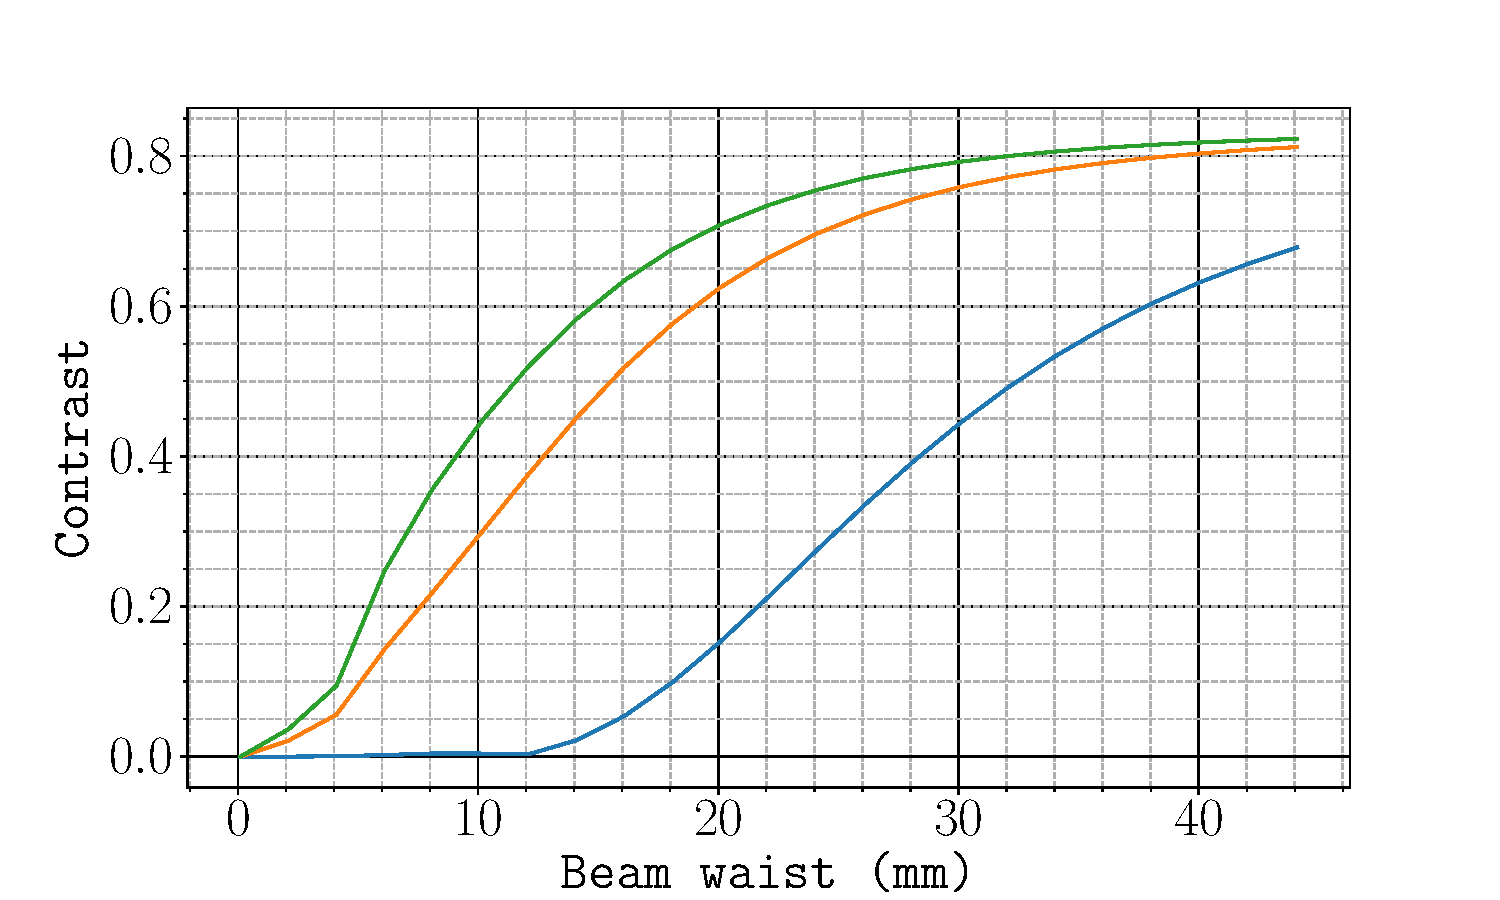
\includegraphics[width=0.7\textwidth]{fringe_contrast.pdf}
	\caption[Simulated fringe contrast vs beam waist size]{Simulated fringe
		contrast as a function of waist size \(w\) for an atom cloud falling under
		gravity. This model assumes a Gaussian distributed atomic density with a
		width \(\sigma_c = \sivalue{5}{\milli\metre}\) and a time between
		interferometer pulses of \(T = \sivalue{25}{\milli\second}\). For smaller
		beam waists the subsequent interferometer pulses have a larger intensity
		gradient across the atom ensemble, which increases the dephasing of the two
		states and reduces the interferometer fringe contrast.}
	\label{fig:raman_fringecontrast}
\end{figure}
\subsection{Wavefront Distortions}\label{subsec:fringe_wavefront}
Another optical effect that influences the
sensitivity is distortions of the laser wavefront. In an ideal case, the
superposition of the counter-propagating spherical wavefronts of the two lasers results in a planar
wavefront for the field that drives the Raman transition. However,
propagation through rough optical elements distort these wavefronts and
introduce a spatially varying component of the Raman phase that is independent
of acceleration. If the atom cloud's trajectory is parallel with the Raman axis,
then this additional phase is the same at each laser pulse and is therefore
cancelled out. 
\par\noindent
On the other hand, this phase is not cancelled when the cloud moves transverse to
the Raman axis. It has the effect of reducing the fringe
contrast. Starting with the assumption that this phase is Gaussian distributed
around 0, with a standard deviation of \(\sigma_\phi\), if this is uncorrelated
at each interferometer pulse, then the interferometer phase \(\Delta \Phi\) will
be distributed with a standard deviation of \(\sigma_\Phi = \sqrt{6}
\sigma_\phi\). Denoting this random phase as \(\delta\phi\), the fringe contrast
is then given by
\begin{equation}
	\mathcal{C}(\delta \phi) = \cos\left(2 \delta\phi\right)
\end{equation}
Following from this, if \( \delta \phi\) is uncorrelated between each atom, the
expected value of the contrast over the ensemble is given by
\begin{align}
	\langle \mathcal{C} \rangle & = \frac{1}{\sqrt{2\pi}\sigma_\Phi}\int \mathcal{C}(\delta \phi) \; e^{-\delta\phi^2/2\sigma_\Phi^2} \; \mathrm{d}\delta\phi \\
	                            & = e^{-2 \sigma_\Phi^2}
\end{align}
\FigureRef{fig:raman_phasenoise} shows the fringe contrast as a
function of this random phase. 
\begin{figure}[htbp]
	\centering
	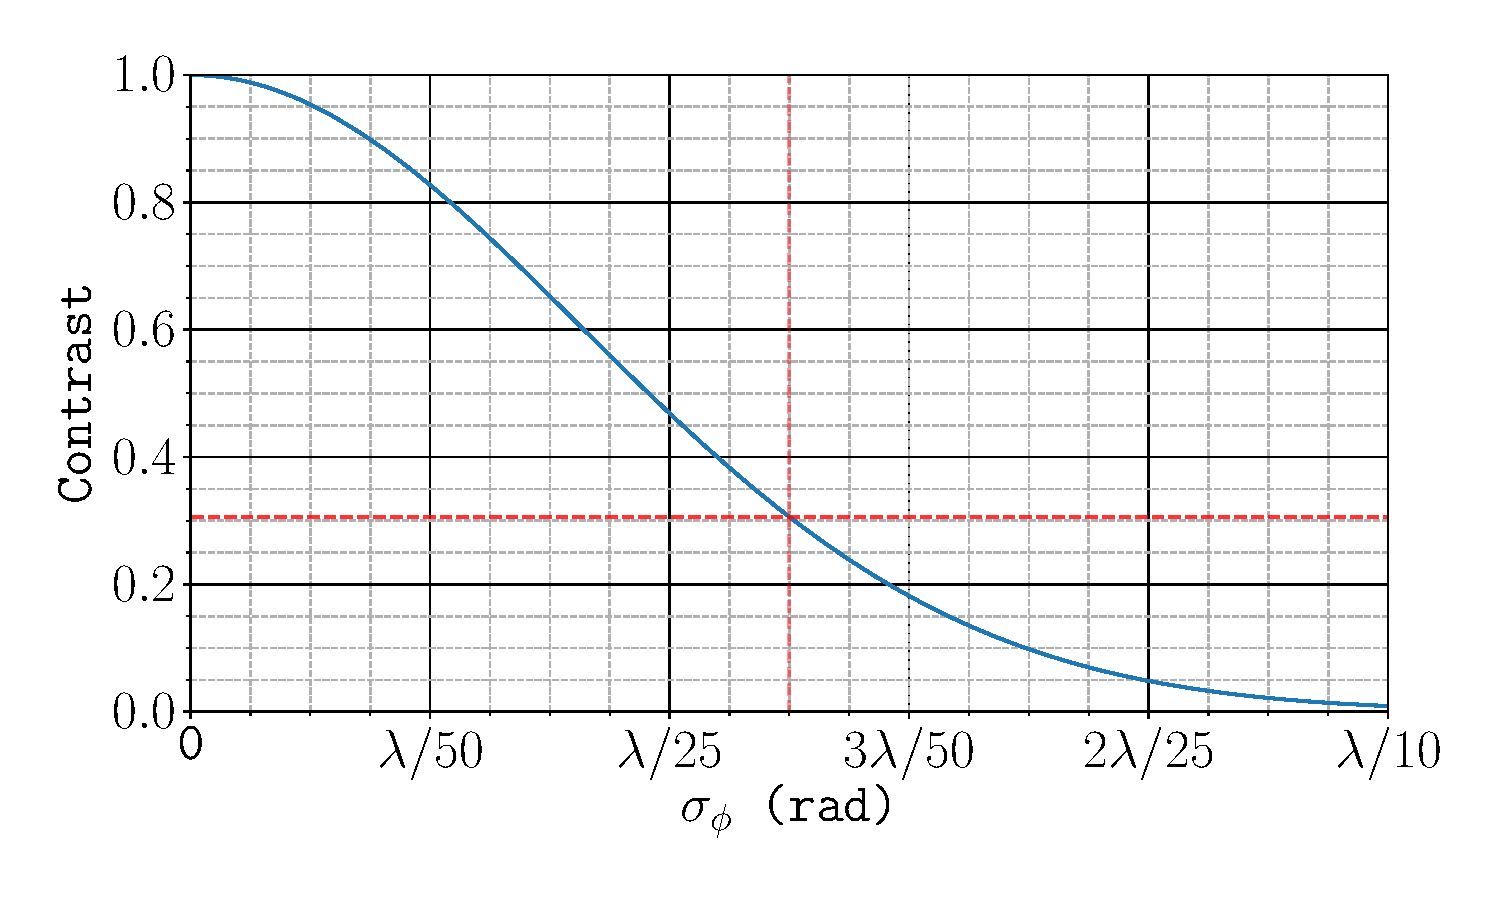
\includegraphics[width=0.7\textwidth]{phase_noise_contrast.pdf}
  \caption[Expected fringe contrast as a function of random phase
  contributions.]{Expected contrast as a function of random phase contributions. This
		assumes that the phase imprinted on an atom during each interferometer pulse
		has an additional random component that is Gaussian distributed around 0
		with a standard deviation of \(\sigma_\phi\). This random phase is also
		uncorrelated between each pulse so that the total can be obtained using
		Gaussian propagation of error. The dashed lines indicate the contrast for
		phase noise expected from conventional optics, which are usually engineered
		to a surface flatness of \(\lambda/20\).}
	\label{fig:raman_phasenoise}
\end{figure}
\par\noindent
This effect is particularly apparent in the context of optical
viewports. The process used to seal an optical viewport to a flange
stresses the glass and distorts its thickness. In fact, commercially
available viewports are specified to give thickness variations up
to $\lambda/20$. At this level, the fringe contrast is severely
reduced.
\par\noindent
A method to systematically characterise this effect has been presented
in~\cite{Schkolnik2015a}. This requires mapping the wavefront
aberrations caused by each optical elements to numerically calculate
their effect on the interferometer phase. This is able to reduce the
uncertainty in their measurement of gravity by an order of
magnitude. For this experiment, the optics for the Raman light were
mounted inside the vacuum chamber to avoid the need for this precise
characterisation. 
\section{Collimation Optics}\label{sec:setup_ramanoptics}
The optical system used to produce the beams for driving Raman transitions,
which will conventionally be referred to as the Raman optics, was designed to
reduce the previously mentioned effects which result in poorer interferometric
fringe visibility and sensitivity to accelerations. Principally, the entire
optical system was mounted inside the optical chamber so that the Raman light
does not pass through any optical viewports before interacting with the atoms.
Typically, the stress placed on the glass during the bonding process will
distort the flatness more than is acceptable for achieving a high contrast. For
example the viewports used for the \ac{mot} optics have a specified flatness of
\(\lambda/4\), so mounting the entire optical system inside the chamber was the
simplest way to avoid a large distortion. 
\subsection{Component Overview}\label{subsec:setup_ramancollimator}
\FigureRef{fig:raman_collimator} presents a diagram of the components used to
send Raman light into the chamber and produce a collimated beam in the centre of
the chamber. The light is coupled into the chamber using a UHV compatible
\ac{pm} fibre, manufactured by Diamond photonics. This is a kapton-coated PM-780
HP fibre that is bonded on one end to a DN16 flange using an epoxy resin. The
external side of this flange has an FC/APC connector for coupling light from
another fibre. Inside the chamber, the ferrule is connected to an FC/APC fibre
plate. This is clamped between a piece which bolts onto the inside of a DN63
flange and another stainless steel plate which bolts onto the rest of the optics
assembly. Fine adjustment of the position of the fibre along the optic axis is
achieved using shim plates with a thickness ranging from
200--\sivalue{300}{\micro\metre}. The fibre plate is free to rotate so that the
orientation of the fibre with respect to a \ac{qwp} at the output of the
collimator. This \ac{qwp} is manufactured by Light Machinery, and is described
further is \SectionRef{subsec:setup_ramanmirror}. When the fibre is correctly
orientated (e.g. when the slow axis of the fibre is at 45\(\deg\) to the slow
axis of the waveplate), the two Raman light fields are orthogonally circularly
polarised. \par\noindent The original design for the optical system consisted of
a triplet lens, as a system of three lenses is capable of correcting for the
five types of Seidel aberrations that distort rays of monochromatic light. This
was designed and manufactured by IC Optical Systems. Another specification for
this lens system was that it had to produce a collimated beam with a waist size
of around \sivalue{35}{\milli\metre} so that the sensitivity of the
interferometer was not limited by the effects of intensity gradients across the
atoms. Unfortunately, the triplet was designed with an incorrect \ac{na}. With a
focal length of \sivalue{123.4}{\milli\metre} and a diameter of
\sivalue{50}{\milli\metre}, the triplet lens has a \ac{na} of 0.194. However,
the nominal \ac{na} for PM780-HP fibre used in the UHV compatible \ac{pm} fibre
is 0.12. Consequently, the light from this fibre did not fill the \ac{na} of the
triplet lens and produced a beam with a waist of 13mm. 
%%{\huge Plot to illustrate this}. 
To address this issue, a pair of aspheric lenses was included to increase
the divergence angle of light from the fibre. These are manufactured by Thorlabs
and have a focal length of \sivalue{4.51}{\milli\metre} (352230-B) and
\(\sivalue{15.29}{\milli\metre}\) (352260-B), respectively, to give a
magnification of 3.39.
\begin{figure}[!htbp]
	\centering
	\def\svgwidth{\columnwidth}
	\subfloat[][]{\scalebox{0.4}{\input{Figures/Chapter6/raman_optics.pdf_tex}\label{fig:raman_collimator}}}
	\subfloat[][]{\scalebox{0.4}{\input{Figures/Chapter6/mirror_mount.pdf_tex}\label{fig:mirror_mount}}}
	\caption[Drawings of the componets used in the Raman optics
		assemblies]{Diagrams of the components used in the Raman optical assemblies.
		(a) shows the collimator setup. Light is coupled into the chamber using a
		UHV fibre feedthrough. A pair of aspheric lenses is used to increase the
		divergence angle of the fibre output, before the light is collimated by a
		triplet lens. Finally, a quarter-wave plate is aligned so that it circularly
		polarises the collimated light fields. (b) illustrates the other half of the
		setup, which is used to retro-reflect the light. A second quarter-wave plate
		is used so that the reflected beams have the same handedness to their
		respected incoming ones. A MEMS accelerometer is mounted on the back of the
		mirror to measure vibrations. These components are all mounted on a
		piezo-controlled mirror mount whose tilt can be controlled from outside the
		vacuum chamber.}
	\label{fig:raman_optics}
\end{figure}
\subsection{Alignment and Collimation}
As one of the main motivations for mounting the Raman optics inside the vacuum
chamber was to reduce the effects of wavefront distortions, it is worth
highlighting how inaccurate alignment of the optics can lead to aberrations. As
previously discussed in \SectionRef{subsec:fringe_wavefront}, distortions of the
wavefront leads to a dephasing and loss of interferometer fringe visibility.
Here, the same figures of merit as before are used to consider what misalignment
is acceptable to ensure that the phase of the Raman wavefront deviates by less
than \(\lambda/100\) after a transverse distance of
\sivalue{12.5}{\milli\metre}. \par\noindent Taking the fibre as a point source,
misalignment can occur if it is displaced from the front focal point of the
optical system longitudinally along or transversely to the optic axis. If it is
transversely displaced, this manifests as an angular displacement of the
collimated light after the triplet lens. A large angular displacement is
undesirable due to the fact that since one of the Raman light fields propagates
further, the two wavefronts that drive acceleration-sensitive Raman transitions
are not parallel. \FigureRef{fig:raman_wave_transverse} shows a simulation of
the wavefront distortion as a result of this transverse misalignment. This is
obtained by simulating the propagation of rays corresponding to each Raman light
field through the optical system. The wavefront is estimated using the slope of
each ray at a distance of \sivalue{43}{\milli\metre} from the output of the
triplet lens, which corresponds to the position of the centre of the vacuum
chamber. The mirror is mounted at the same distance from the centre, so the
second beam propagates \sivalue{129}{\milli\metre}. Close to the optic axis,
this distortion is approximately linear (i.e. a tilt) and it can be seen that a
displacement of the fibre from the optic axis of <\sivalue{1}{\milli\metre} is
sufficient to achieve the desired wavefront flatness. \par\noindent Aside from a
transverse displacement, it is possible that the fibre could be misaligned along
the optic axis. In which case, the output beam will not be collimated.
Consequently, the counter-propagating reflected rays will not be antiparallel to
incoming ones. The effect of this longitudinal displacement on the Raman
wavefront is shown in~\FigureRef{fig:raman_wave_longitudinal}. Further from the
optic axis the deviation in the phase of the light is greater, giving a
quadratic distortion which is characteristic of a defocus. Comparing the
wavefront distortion in this case, a requirement on the longitudinal
misalignment of \(< \sivalue{0.6}{\milli\metre}\) is needed for the previously
specified flatness.

\begin{figure}[!htbp]
	\centering
	\def\svgwidth{\columnwidth}
	\subfloat[][]{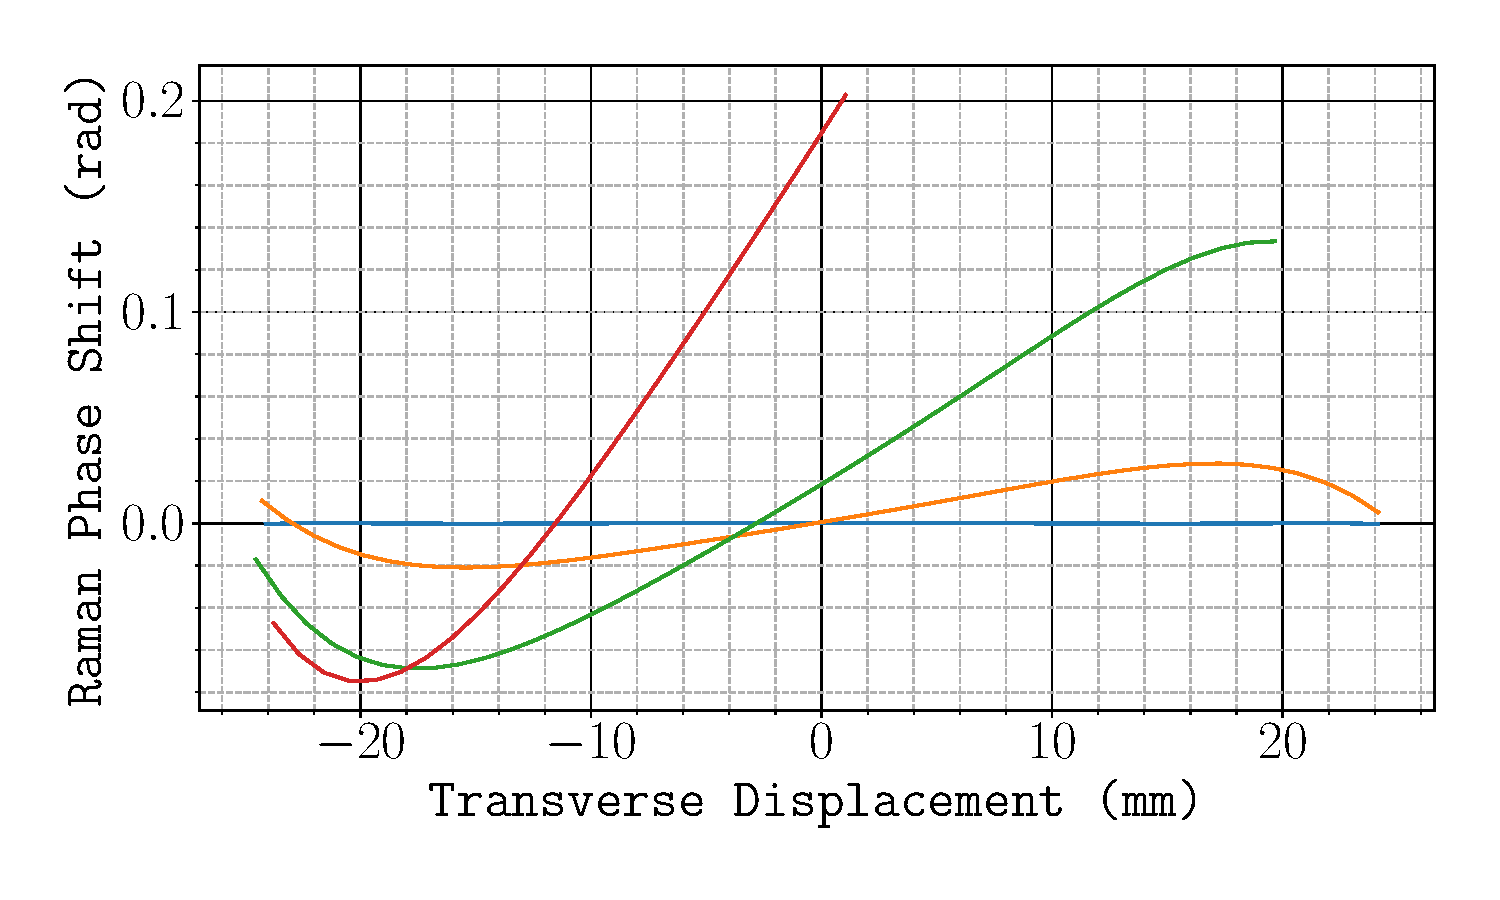
\includegraphics[width=0.4\textwidth]{wavefront_transverse.pdf}\label{fig:raman_wave_transverse}}
	\subfloat[][]{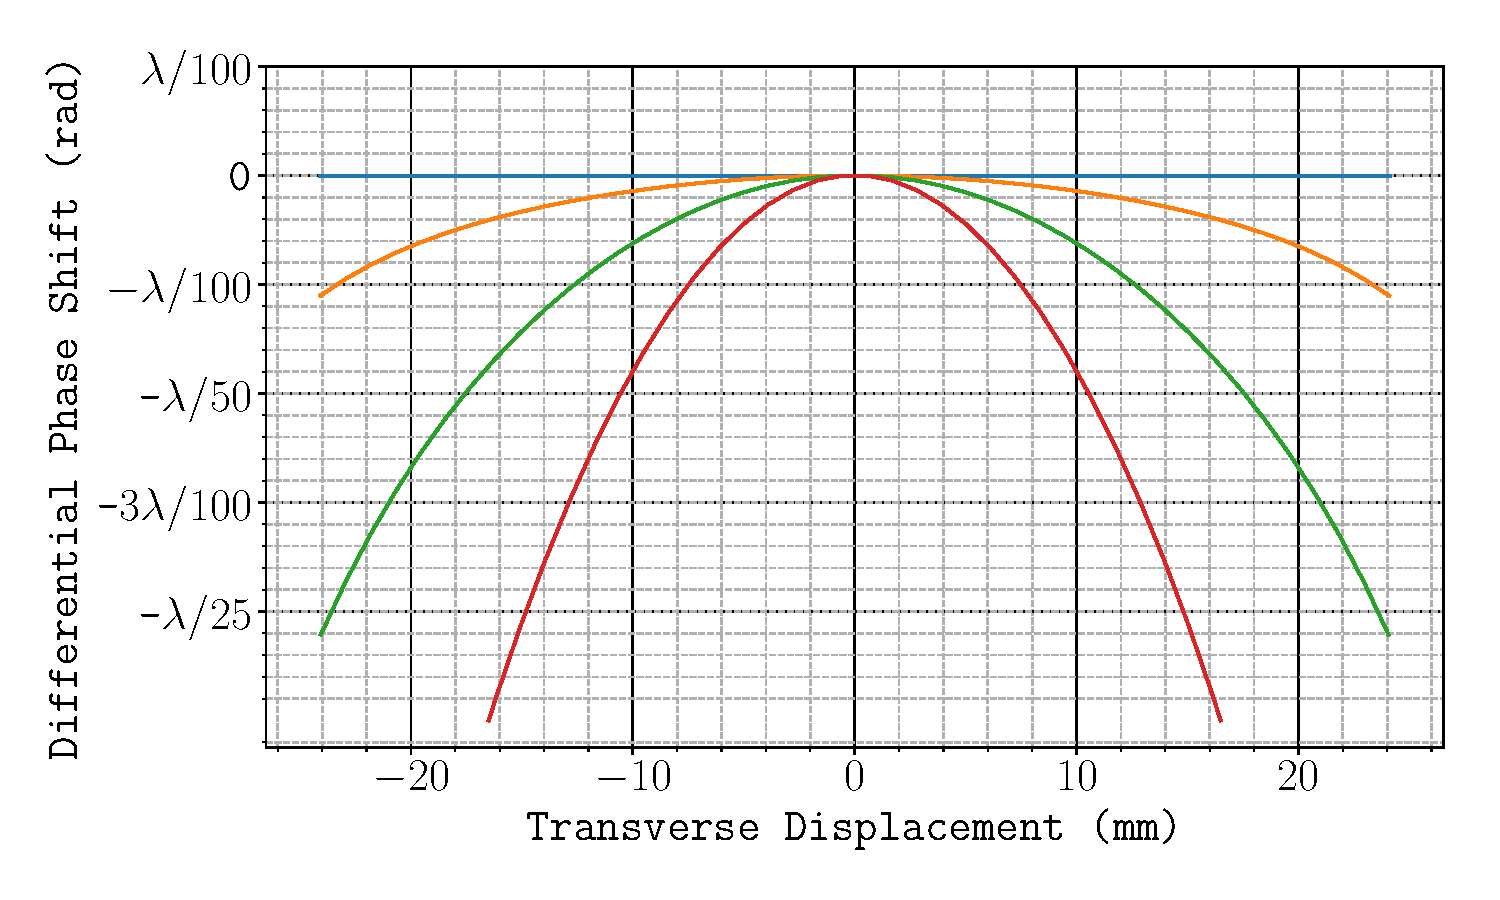
\includegraphics[width=0.4\textwidth]{wavefront_longitudinal.pdf}\label{fig:raman_wave_longitudinal}}
	\caption[Simulated wavefront distortion for longitudinal and transverse fibre
		misalignment]{Simulated wavefront distortion for longitudinal and transverse
		fibre misalignment. Rays from a point source with a divergence angle
		corresponding to a \ac{na} of 0.12 are propagated through the Raman optical
		system. Rays corresponding to the reflected beam are propagated further with
		the assumption that the mirror is perpendicular to the optic axis. The first
		set of rays propagates \sivalue{43}{\milli\metre} and the second propagates
		\sivalue{129}{\milli\metre}. The wavefront for each beam is calculated by
		taking the slope of each ray and subtracting from the slope of the central
		ray. The wavefront of the effective field that drives the Raman transition
		is the difference of these two wavefronts. (a) shows the distortion of the
		wavefront for a transverse misalignment of the fibre for a displacement of
		\sivalue{0}{\milli\metre} (blue), \sivalue{0.5}{\milli\metre} (orange)
		\sivalue{1}{\milli\metre} (green) and \sivalue{1.5}{\milli\metre} (red) from
		the front focal point. (b) shows the wavefront for longitudinal
		displacements of \sivalue{0}{\milli\metre} (blue),
		\sivalue{0.3}{\milli\metre} (orange)
		\sivalue{0.6}{\milli\metre} (green) and \sivalue{1}{\milli\metre}
		(red).}\label{fig:fig_label}
\end{figure}
\subsection{Measuring the Beam Width}
To measure the waist of the beam, its reflection from a flat surface was imaged
using a CCD camera. The radius of the triplet lens is smaller than the beam
waist, so the beam is apertured by this lens. To take account of this aperture,
the beam waist was estimated using a Taylor expansion of a Gaussian to second
order:
\begin{align}
	I(x) & = A e^{-\frac{(x-x_0)^2}{2 w^2}} \nonumber                                                                              \\
	     & \approx A-\frac{2 A x_0^2}{w^2}+\frac{4 A x x_0}{w^2}-\frac{2 A x^2}{w^2} + \mathcal{O}(x^3) \label{eq:gaussian_approx}
\end{align}
A typical intensity profile along the horizontal and vertical camera axes is
shown in~\FigureRef{fig:beam_examp}. A threshold intensity value excludes
contributions from pixels outside of the spatial extent of the beam. The waist
was estimated using a linear least-squares fit of the intensity profile to a
second-order polynomial \(c_0 + c_1 x + c_2 x^2\), where \begin{equation} w =
\left|\frac{\sqrt{c_1^2-4c_0 c_2}}{\sqrt{2}c_2} \right| \end{equation} A plot of
the estimated beam waist over a propagation distance of \sivalue{1}{\metre} is
shown in~\FigureRef{fig:beam_waist}. Inside the chamber each Raman beam
propagates \sivalue{5.25}{\centi\metre} and \sivalue{15.75}{\centi\metre}, where
the beam is well collimated. Along the vertical axis, the beam has a waist of
around \sivalue{36.9}{\milli\metre}. The horizontal waist is smaller because the
camera was horizontally tilted from the beam's optic axis. The projection of the
beam onto this axis is consistent with a horizontal tilt of
\sivalue{16}{\degree}.  \begin{figure} \centering
	\def\svgwidth{\columnwidth}
	\subfloat[][]{\scalebox{0.3}{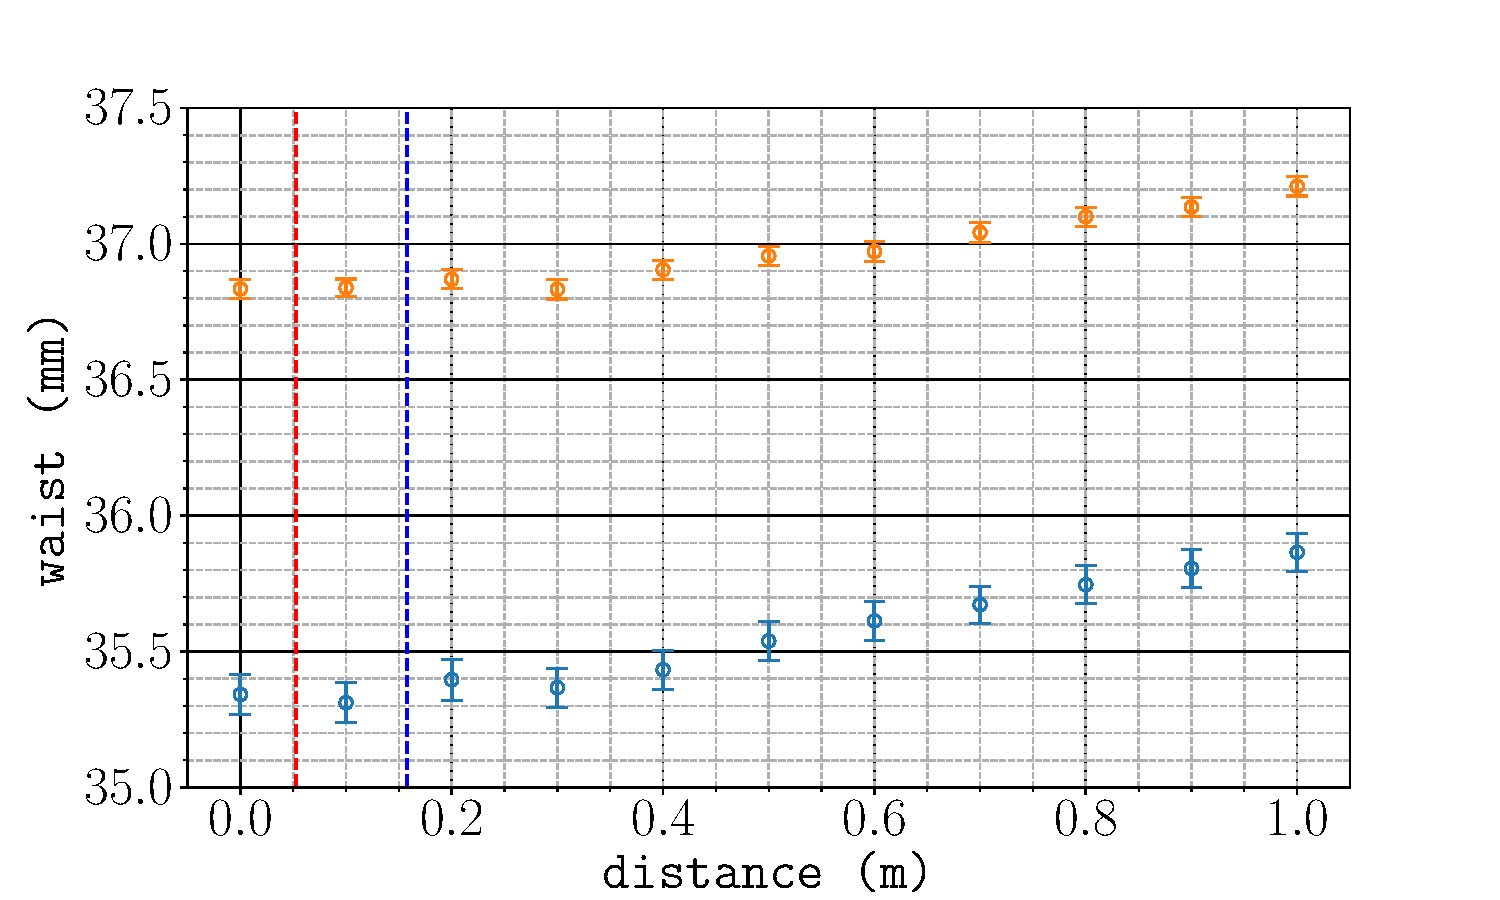
\includegraphics{beam_waist}}\label{fig:beam_waist}}
	\subfloat[][]{\scalebox{0.3}{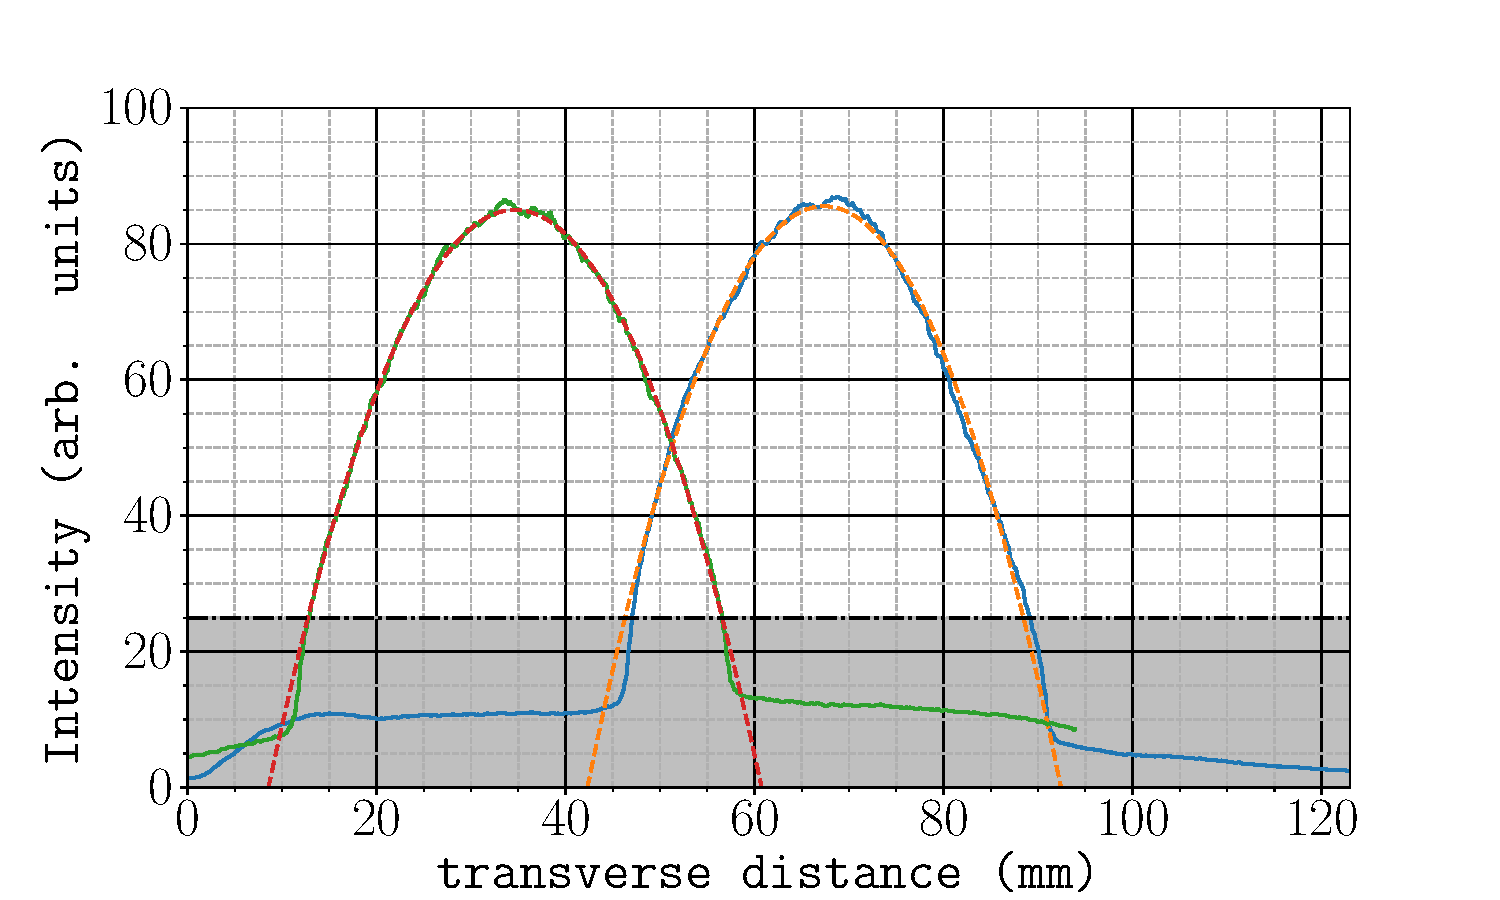
\includegraphics{beam_examp}}\label{fig:beam_examp}}
	\caption[Measured Raman beam waist]{Raman beam waist measured over a distance
		of \sivalue{1}{\metre}, shown in \textbf{(a)}. The waist along the
		horizontal and vertical axes are indicated in blue and orange respectively.
		The dashed lines indicate the approximate propagation distance of each beam
		at the position of the atoms. \textbf{(b)} shows the intensity profile along
		each axis, with the fitted parabola. The dot-dashed line is a threshold
		intensity value, which excludes pixels from outside the spatial extent of
		the beam.} 
  \label{fig:beam_waist_plots} 
\end{figure}
\section{Retro-Reflection Assembly}\label{subsec:setup_ramanmirror} The
		Raman transitions used in the interferometer are driven by
		counter-propagating light fields to give a large momentum transfer of \(2
		\hbar k\) to the atoms. The two beams enter from the same fibre input, so a
		mirror is used to retro-reflect them. The retro-reflection assembly includes
		a \ac{qwp} to ensure that the reflected beams have the same polarisation
		handedness as their circularly polarised incoming counterpart. \par\noindent
		The mirror is also manufactured by Light Machinery, and the \ac{qwp} is made
		to the same specifications as the one that circularly polarises the incoming
		beams.  During the manufacturing process, the waveplates and mirror were
		polished to reduce irregularities in the thickness of each \ac{qwp} and the
		surface of the mirror. \FigureRef{fig:waveplate_map} shows the variation in
		the thickness of the waveplate in front of the triplet lens, measured by
		Light Machinery using a white light interferometer. This has a standard
		deviation of \sivalue{4.62}{\nano\metre} and corresponds a standard
		deviation of the optical path length of \pow{8.6}{-3}\(\lambda\).
\begin{figure}[!htbp] 
  \centering
  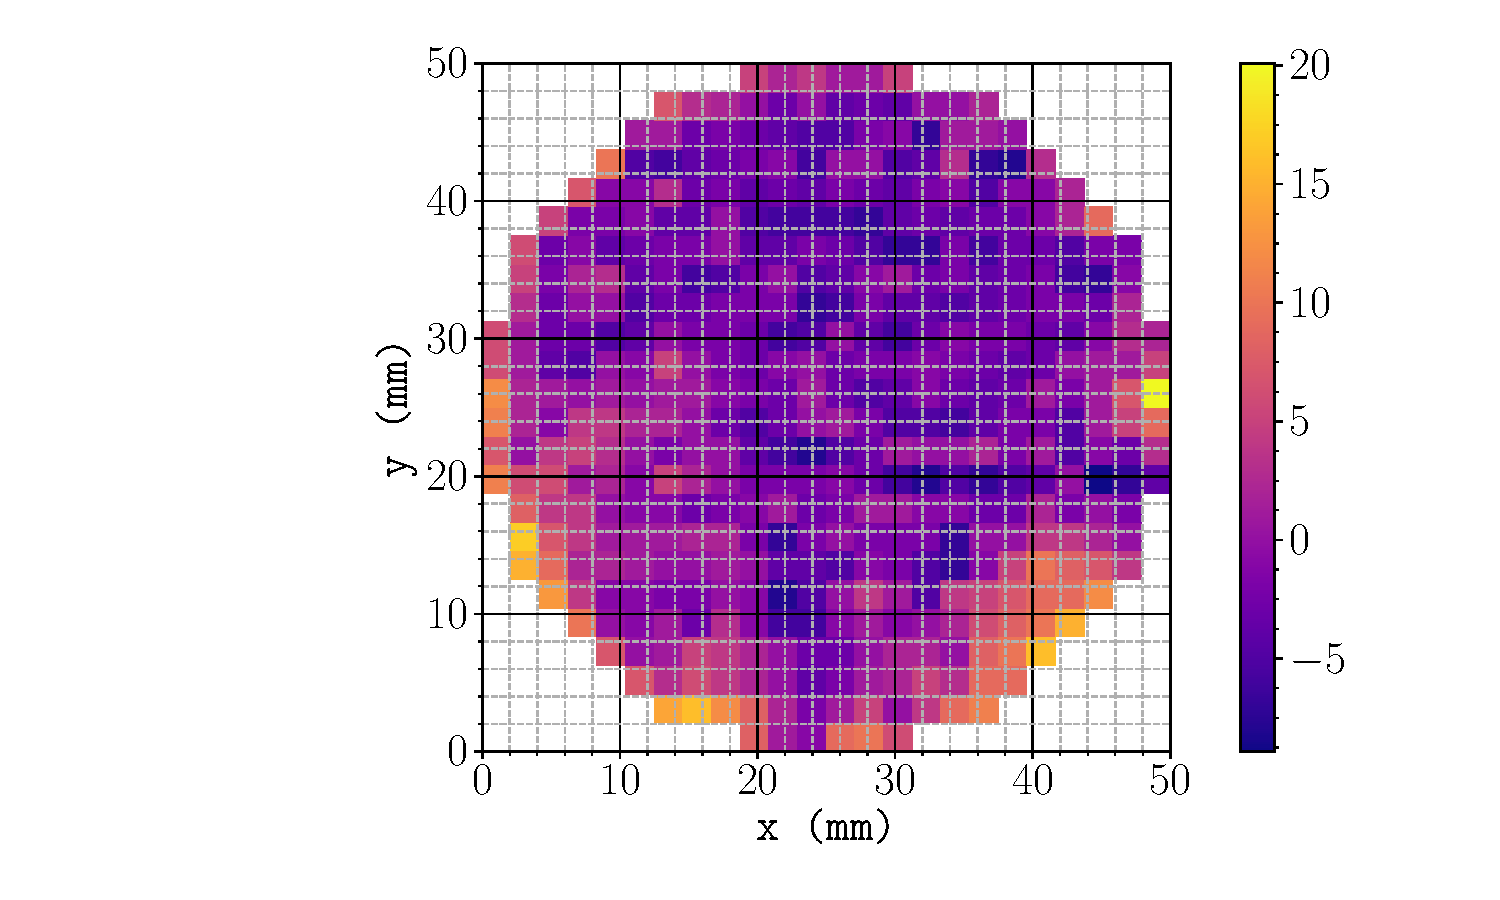
\includegraphics[width=0.7\textwidth]{waveplate.pdf}
  \caption[Quarter-wave plate thickness variation.]{Thickness of the first \ac{qwp}, measured by a white light
		interferometer. The value is given in \sivalue{}{\nano\metre} as a
		difference from the mean thickness. The standard deviation of this thickness
		is \sivalue{4.62}{\nano\metre} and a peak-to-valley (PV) of {\textbf need
		number here}. Equivalent surface data for the other \ac{qwp} and mirror were
		not provided by Light Machinery, but had a PV thickness variation of
		\sivalue{19}{\nano\metre} and
		\sivalue{9}{\nano\metre} respectively.} \label{fig:waveplate_map}
\end{figure} 
The \ac{qwp} and mirror are fixed onto the front
plate of a UHV compatible MDI-HS mirror mount, manufactured by Radiant dye. The
horizontal and vertical tilt of the mirror can be adjusted using two thumbscrew
actuators which cause the front plate to pivot around a ball bearing. This mount
is designed for high stability, but of course the alignment will still drift
over time. To avoid the need to periodically open the chamber to realign the
mirror, a piezo-electric stack is placed between each actuator and the front
plate so that the tilt of the mirror can be adjusted externally. Each
piezo-stack is connected to a high-voltage feedthrough, so that their length
(and hence mirror tilt) can be finely adjusted by controlling the voltage
applied across them. A control voltage ranging between 0--\sivalue{10}{\volt} is
amplified by a controller to give an applied voltage across the piezo stack
between -10--\sivalue{150}{\volt}. This corresponds to a travel range of
\sivalue{23}{\micro\metre}. \par\noindent To understand the effect of
misalignment, it is instructive to consider its effect on the effective
wavevector \(\keff\). If the
mirror is misaligned from the incoming beam's wavevector by an angle
\(\theta\),
the two counter-propagating fields that drive Raman transitions have wavevectors
\(k_1 \left(1,0\right)\) and \(k_2 \left(\cos(\theta),\sin(\theta)\right)\).
\(\keff = {\textbf k_1} - {\textbf k_2} \cos (2\theta_i)\). Fortunately, for
small angular displacements, i.e. \(< \sivalue{1}{\milli\radian}\), this does
not greatly reduce the sensitivity to accelerations. In short, this means that
\(\keff\) will have a spatially varying direction. Since an atom interacting via
a Raman transition picks up a phase \(\phi = \keff . {\textbf x}\), atoms
travelling along different trajectories will accumulate different phases due to
the spatial variation of \(\keff{}\). Across the atom ensemble, this leads to a
dephasing and consequently, a loss of interferometer fringe
visibility~\cite{Tackmann2012} 
\subsection{In-Situ Alignment and Optimisation} 
After mounting the Raman optical system inside the chamber, the
mirror had to be aligned to retro-reflect the light. When the mirror is close to
perpendicular to the light's wavevector, some of the power in the reflected beam
couples back into the fibre. In principle, this power is maximised when the
mirror is exactly perpendicular so maximising this power is a useful technique
to align the mirror. A 99:1 fibre splitter was used to couple light into the
chamber, which provided a means to measure the back-reflected power without
needing any free-space optics. This was set up so that 99\% of the incoming
light entered the chamber, with the other 1\% coupled into the corresponding
output port. Due to the fact that a beam-splitter acts reversibly, 1\% of the
back-reflected light which couples into vacuum fibre exits the fibre-splitter on
the other input port. Therefore, the power at this output was used to indirectly
measure the alignment of the mirror.  
\par\noindent 
The travel range of the piezo stacks does not cover the full motional
range of the mirror mount. It was initially coarsely aligned using the
thumbscrew actuators.
Once
installed, the lack of direct access to optical system meant that conventional
methods to coarsely align the mirror, such as observing the location of the
reflected beam's focus, were not feasible. Rather than carry out the somewhat
tedious job of systematically adjusting each thumbscrew until the mirror was
aligned, an automatic routine was devised to do this. This was carried out using
a pair of bipolar stepper motors that each rotated a ball driver inserted into
the head of each thumbscrew. The revolution of these motors was controlled using
an Arduino microcontroller, which communicated to the computer using a serial
interface.  The motors rotated by 0.9\(\deg\)/step, which corresponds to a tilt
of the mirror by \sivalue{18.1}{\micro\radian}. This is smaller than the
\sivalue{0.67}{\milli\radian} angular displacement that the piezo stack could
provide, but the slow execution speed of the motor control meant that it was
more practical to use a combination of the motors and piezos to systematically
scan through the tilt of the mirror mount.  %%{\textbf {huge find out how big spot size was }}. 
\par\noindent 
Using this method, the mirror mount was aligned so
that the maximum of the back-reflected power was reachable with the piezo
stacks. Of course, it was foreseeable that the mirror would need to be
periodically realigned, which would require another systematic iteration through
the voltages applied to each piezo stack. Given that this search was quite time
consuming, it was not a practical way to maintain alignment. To improve upon
this, an optimisation method using the Nelder-Mead simplex
algorithm~\cite{Nelder1965} was implemented. This method is suitable for
optimising multidimensional functions and has been used to demonstrate the
automatic alignment of a fibre with up to 6 degrees of freedom~\cite{Zhang2004}.
\par\noindent
The Nelder-Mead algorithm aims to optimise the value of an objective
function (in this instance, the optical power measured as a voltage by a
photodiode) by sampling the function at various locations. For \(n\) parameters,
a set of \(n-1\) points distributed randomly across the parameter space are
chosen as the initial simplex. These are sorted in decreasing order of the value
of the objective function and the algorithm proceeds by performing geometric
transformations on this simplex, by sequentially reflecting, expanding and
contracting this simplex. Each step starts with a reflection about the line
between the two greatest values. The coordinates of the simplex are updated if
the function has a greater value at the location given by one of these
transformations, until the algorithm converges on a maximum value. As with many
optimisation algorithms, the Nelder-Mead method has the potential to converge on
a local optimum, but this is alleviated by expanding the simplex to look for
more optimal values. The termination of the algorithm was decided by using the
standard deviation of the last 5 values. Empirically, it was found that
terminating when the standard deviation was less than \sivalue{10}{\micro\volt}
resulted in stable performance of the algorithm, even when the signal-to-noise
ratio of the measured voltage was poor. An example of this algorithm aligning
the mirror mount is presented in \FigureRef{fig:simplex_optimisation}. To verify
that the converged value was optimal, a systematic scan of the piezo stack
control voltages in the region around this value was also carried out. In this
case, the algorithm converged on a local maximum, but one that greatly enhanced
the coupling efficiency of the reflected light back into the fibre. The
difference in the piezo control voltages from their optimal values corresponds
to a tilt of the mirror mount along the horizontal and vertical axis of less
than \sivalue{13}{\micro\radian}.  
\begin{figure}[!htbp] 
  \centering
	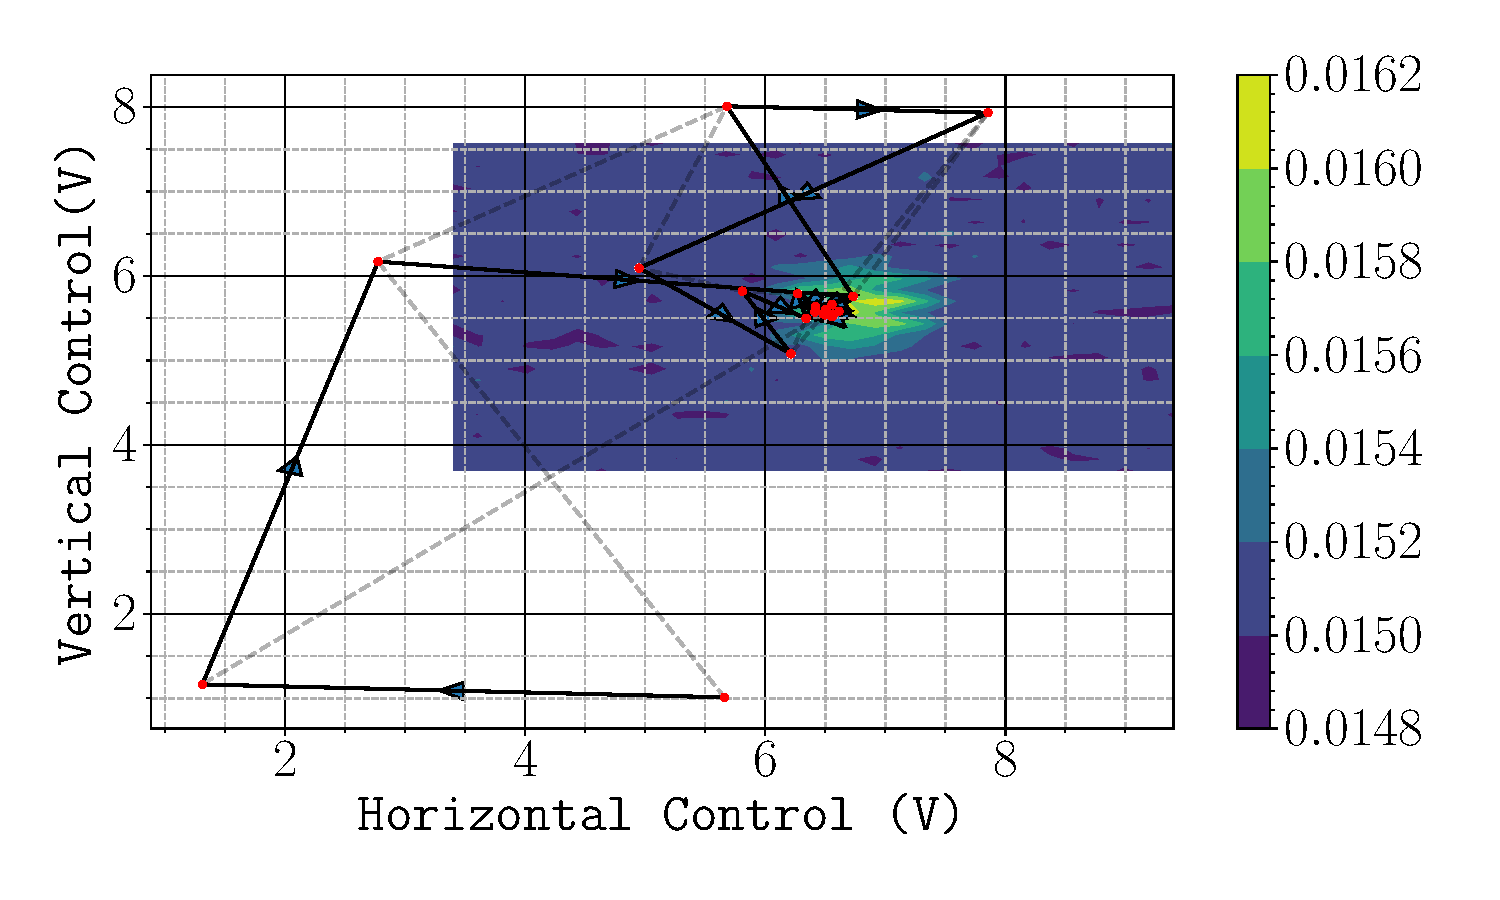
\includegraphics[width=0.7\textwidth]{simplex_alignment}
	\caption[Automatic mirror alignment using the Nelder-Mead simplex
		algorithm.]{Automatic mirror alignment using the Nelder-Mead simplex
		algorithm. A sequence of geometric transformations on the initial
    simplex are used to converge on the optimum point, where the
    back-reflected power is maximised. The shaded lines indicate the simplex bounded by
    the three co-ordinates at each iteration.
		A raster scan of the piezo control
		voltages close to the optimum is also plotted. The irregular shape of the
		measured power is a result of a hysteresis effect when the horizontal
		control voltage was changed from its maximum value to the minimum.}
		\label{fig:simplex_optimisation} 
  \end{figure}
\subsection{The Mechanical Accelerometer}\label{subsec:raman_mems}
The periodic interferometer signal means that the interferometer phase is only
proportional to acceleration over one fringe spacing \(\Delta a =
\frac{\pi}{\keff T^2}\). Furthermore, the fringe spacing is inversely
proportional to \(T^2\) so there is a trade-off between dynamic range and
sensitivity. These problems can be addressed by making use of a mechanical
accelerometer mounted onto the back of the retro-reflecting mirror to form a
hybrid system~\cite{Lautier2014}. The accelerometer determines the acceleration
up to the fringe spacing  and the interferometer measures the acceleration more
precisely. The accelerometer also measures the vibrations of the
retro-reflecting mirror, so it can be used to filter the effects of vibration
noise on the interferometer signal. This is discussed in more detail
in~\SectionRef{subsec:vibration_sensitivity}. This hybridisation scheme has been
used in measurements of gravity in high noise environments such as the centre of
Paris~\cite{Merlet2009} and in parabolic aircraft
flights~\cite{Geiger2011a,Barrett2016}. \par\noindent The accelerometer is a
navigation-grade AI-Q-2010 manufactured by \textit{Innalabs}. This particular
device was chosen because its specified intrinsic noise was
<\sivalue{7}{\micro\g} in the 0-\sivalue{100}{\Hertz} bandwidth. For a pulse separation \(T
= \sivalue{25}{\milli\second}\), the fringe spacing is
\(\sivalue{31.2}{\micro\g}\) so it is sensitive enough to measure the
acceleration to within one fringe. A schematic of this device is shown
in~\FigureRef{fig:innalabs}. It operates using a quartz pendulum which is is
free to move about one axis~\cite{Foote1992}. Under an acceleration, the
deflection of the pendulum is capacitively detected. A servo loop circuit drives
a current through the coils to restore the position of the pendulum. This
current is directly proportional to the acceleration of the pendulum. This model
has a nominal scale factor of \sivalue{1.235976}{\milli\ampere\per\g}. The
acceleration is measured using a load resistance of \sivalue{6}{\kilo\ohm} to
give an output voltage of \sivalue{7.56}{\volt\per\g}.
\begin{figure}[!htbp] \centering
	\resizebox{0.5\textwidth}{!}{\input{innalabs.pdf_tex}}
	\caption[Innalabs accelerometer cross-section]{Cross-section of the Innalabs
		AI-Q-2010 accelerometer.} \label{fig:innalabs}
\end{figure}

\section{Conclusion}
This chapter has motivated the need for low wavefront distortions to achieve sensitive measurements of acceleration, particularly when there is significant transverse motion across the Raman beam. Following this, the in-vacuum optical system was introduced. This helps to reduce the effect of wavefront distortions by not transmitting the beam through an optical viewport. Finally, the retro-reflection assembly used to produce the counter-propagating beams has been presented.  
